\section{Introducción}

\begin{frame}\frametitle{Algunos conceptos previos}
    \begin{itemize}
  \item \textbf{Configuración:} es la descripción de la posición en el espacio de todos los puntos del robot. Se denota con $q$.
  \item \textbf{Espacio de configuraciones:} es el conjunto $Q$ de todas las posibles configuraciones. 
  \item \textbf{Grados de libertad:} número mínimo de variables independientes para describir una configuración. En este curso, la base móvil del robot tiene 3 GdL, la cabeza tiene 2 GDL y cada brazo tiene 7 GDL más 1 GdL para el gripper. En total, el robot tiene 21 GdL. 
  \end{itemize}
  \textbf{Propiedades del robot:}
  \begin{itemize}
  \item \textbf{Holonómico:} el robot puede moverse instantáneamente en cualquier dirección del espacion de configuraciones. Comunmente se logra mediante ruedas de tipo \textit{Mecanum} u \textit{Omnidireccionales}. 
  \item \textbf{No holonómico:} existen restricciones de movimiento en velocidad pero no en posición. Son restricciones que solo se pueden expresar en términos de la velocidad pero no pueden integrarse para obtener una restricción en términos de posición. Ejemplo: un coche sólo puede moverse en la dirección que apuntan las llantas delanteras, sin embargo, a través de maniobras puede alcanzar cualquier posición y orientación. El robot de este curso es no holonómico. 
  \end{itemize}
\end{frame}

\begin{frame}\frametitle{Algunos conceptos previos}
  \textbf{Propiedades de los algoritmos:}
  \begin{itemize}
  \item \textbf{Complejidad:} cuánta memoria y cuánto tiempo se requiere para ejecutar un algoritmo, en función del número de datos de entrada (número de grados libertad, número de lecturas de un sensor, entre otros).
  \item \textbf{Optimalidad:} un algoritmo es óptimo cuándo encuentra una solución que minimiza una función de costo.
  \item \textbf{Completitud:} un algoritmo es completo cuando garantiza encontrar la solución siempre que ésta exista. Si la solución no exite, indica falla en tiempo finito.
    \begin{itemize}
    \item Completitud de resolución: la solución existe cuando se tiene una discretización. 
    \item Completitud probabilística: la probabilidad de encontrar la solución tiende a 1.0 cuando el tiempo tiende a infinito.
    \end{itemize}
  \end{itemize}
\end{frame}

\begin{frame}\frametitle{Planeación de movimientos}
El problema de la planeación de movimientos comprende cuatro tareas principales:
  \begin{itemize}
  \item Mapeo: construir una representación del ambiente a partir de las lecuras de los sensores y la trayectoria del robot.
  \item Navegación: encontrar un conjunto de puntos $q \in Q_{free}$ que permitan al robot moverse desde una configuración inicial $q_{start}$ a una configuración final $q_{goal}$.     
  \item Localización: determinar la configuración $q$ dado un mapa y lecturas de los sensores. 
  \item Barrido: pasar un actuador por todos los puntos $q\in Q_b \subset Q$.
  \end{itemize}
\end{frame}

\section{Representación del ambiente}
\begin{frame}\frametitle{Representación del ambiente}
  Un mapa es cualquier representación del ambiente útil en la toma de decisiones.
  \begin{itemize}
  \item Interiores (se suelen representar en 2D)
    \begin{itemize}
    \item Celdas de ocupación
    \item Mapas de líneas
    \item Mapas topológicos: Diagramas de Voronoi generalizados. 
    \item Mapas basados en \textit{Landmarks}
    \end{itemize}
  \item Exteriores (suelen requerir una representación 3D)
    \begin{itemize}
    \item Celdas de elevación
    \item Celdas de ocupación 3D
    \item Octomaps
    \end{itemize}
  \end{itemize}
\end{frame}

\begin{frame}\frametitle{Celdas de ocupación}
  Es un tipo de mapa geométrico. El espacio se discretiza con una resolución determinada y a cada celda se le asigna un número $p\in[0,1]$ que indica su nivel de ocupación. En un enfoque probabilístico este número se puede interpretar como la certeza que se tiene de que una celda esté ocupada.
  \begin{figure}
    \centering
    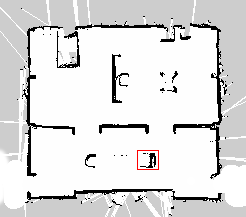
\includegraphics[width=0.4\textwidth]{Figures/MotionPlanning/OccupancyGrid.png}
    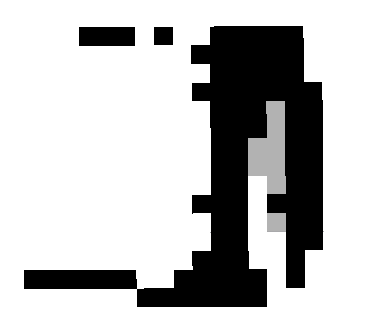
\includegraphics[width=0.4\textwidth]{Figures/MotionPlanning/OccupancyGridZoom.png}
    \end{figure}
  El mapa resultante se representa en memoria mediante una matriz de valores de ocupación. En ROS, los mapas utilizan el mensaje \texttt{nav\_msgs/OccupancyGrid}.
\end{frame}

\begin{frame}\frametitle{Inflado de celdas de ocupación}
  Aunque las celdas de ocupación representan el espacio donde hay obstáculos y donde no, en realidad, el robot no puede posicionarse en todas las celdas libres, debido a su tamaño, como se observa en la figura:
  \begin{columns}
    \begin{column}{0.6\textwidth}
      \begin{figure}
        \centering
        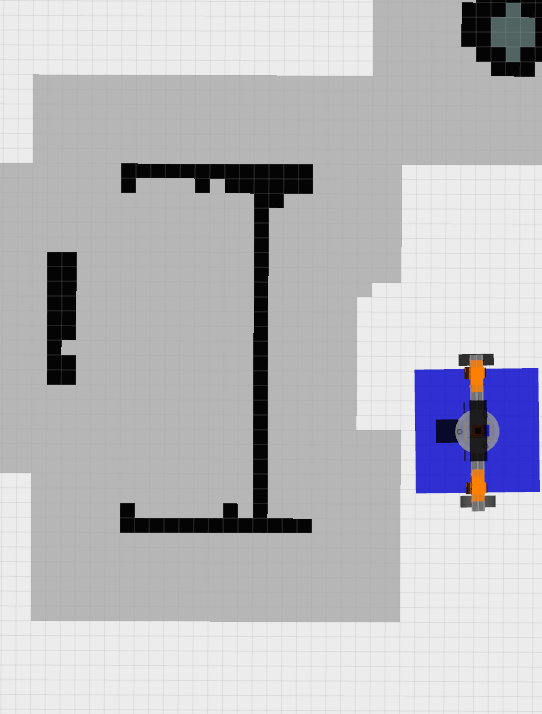
\includegraphics[width=0.45\textwidth]{Figures/MotionPlanning/InflationExample1.png}
        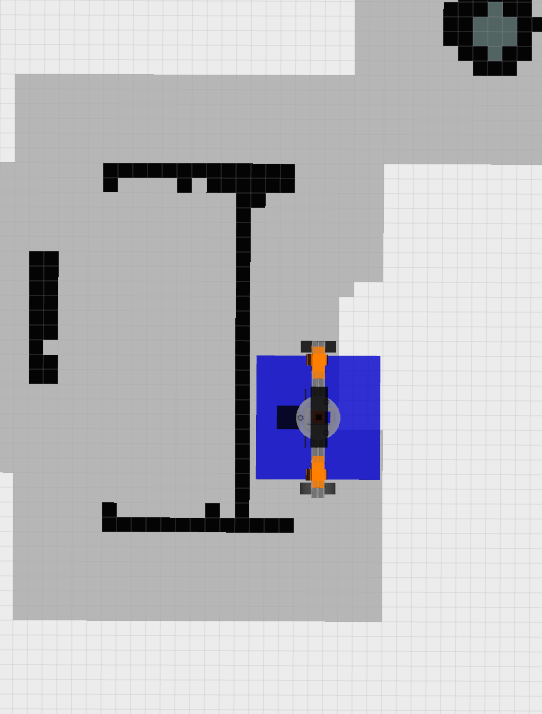
\includegraphics[width=0.45\textwidth]{Figures/MotionPlanning/InflationExample2.png}
      \end{figure}
    \end{column}
    \begin{column}{0.4\textwidth}
      \begin{itemize}
      \item Celdas blancas: espacio libre.
      \item Celdas negras: espacio con obstáculos.
        \item Celdas grises: espacio sin obstáculos donde el robot no puede estar debido a su tamaño. 
      \end{itemize}
    \end{column}
  \end{columns}
  \begin{itemize}
  \item Un mapa de celdas de ocupación debe \textit{inflarse} antes de usarse para planear rutas.
  \item Esta operación se conoce como \textit{dilatación} y es tipo de \textit{operador morfológico}
  \item El inflado se usa para planeación de rutas, no para localización.
  \end{itemize}
\end{frame}

\begin{frame}\frametitle{Diagrama de Voronoi Generalizado}
  \begin{itemize}
  \item A diferencia de los mapas geométricos, donde se busca reflejar la forma exacta del ambiente, los \textbf{mapas topológicos} buscan representar solo las relaciones espaciales de los puntos de interés.
  \item Los Diagramas de Voronoi dividen el espacio en regiones. Cada región está asociada a un punto llamado semilla, sitio o generador. Una región asociada a una semilla $x$ contiene todos los puntos $p$ tales que $d(x,p)$ es menor o igual que la distancia $d(x^\prime, p)$ a cualquier otra semilla $x^\prime$.
  \item Un diagrama de Voronoi generalizdo (GVD) considera que las semillas pueden ser objetos con dimensiones y no solo puntos. 
  \end{itemize}
  \begin{figure}
    \centering
    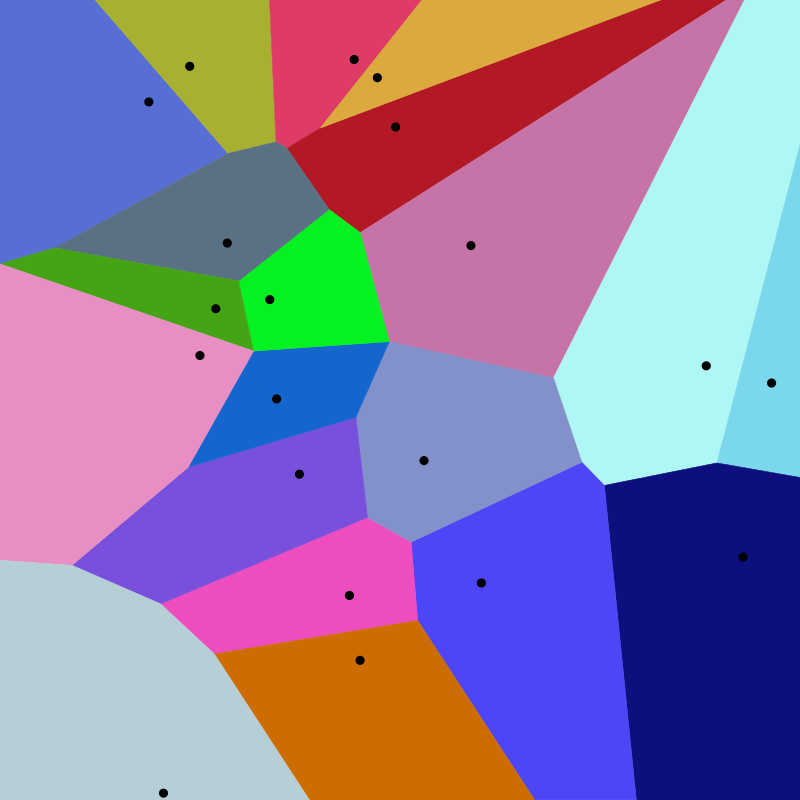
\includegraphics[height=0.4\textheight]{Figures/MotionPlanning/GVD.png}
    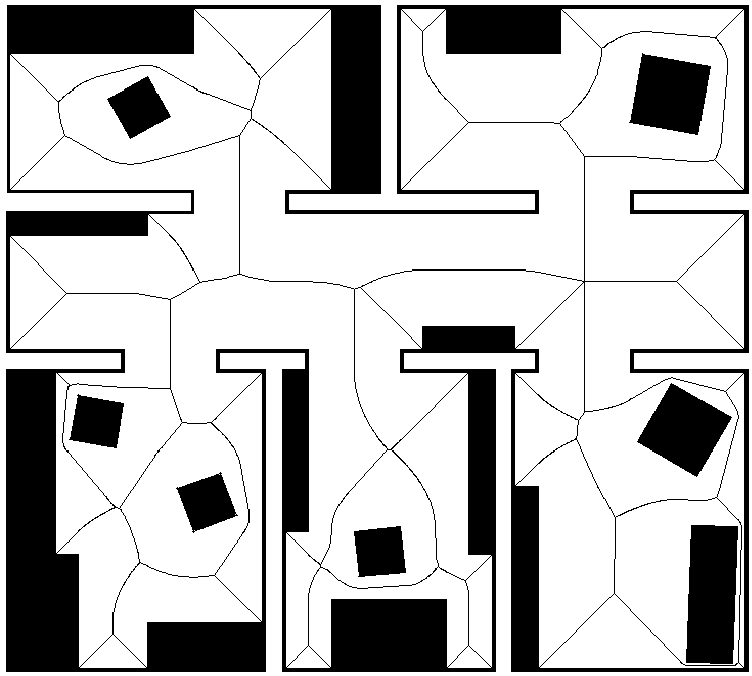
\includegraphics[height=0.4\textheight]{Figures/MotionPlanning/GVDExample.png}
  \end{figure}
  \begin{itemize}
    \item La forma de las regiones depende de la función de distancia que se utilice. 
  \end{itemize}
\end{frame}

\begin{frame}\frametitle{El algoritmo \textit{Brushfire}}
  \begin{columns}
    \begin{column}{0.65\textwidth}
      \begin{itemize}
      \item Obtener un GVD es aún un problema abierto
      \item Se simplifica el problema si se asume un espacio finito y discretizado (celdas de ocupación)
      \item En este caso el GVD se puede obtener mediante el algoritmo \textit{Brushfire}
      \item El mapa de rutas mostrado en la figura se forma con las celdas que son máximos locales en el mapa de distancias devuelto por Brushfire, es decir, son las celdas que son fronteras entre las regiones de Voronoi.
      \item Estas celdas también son aquellas equidistantes a los dos obstáculos más cercanos. 
      \end{itemize}
    \end{column}
    \begin{column}{0.35\textwidth}
      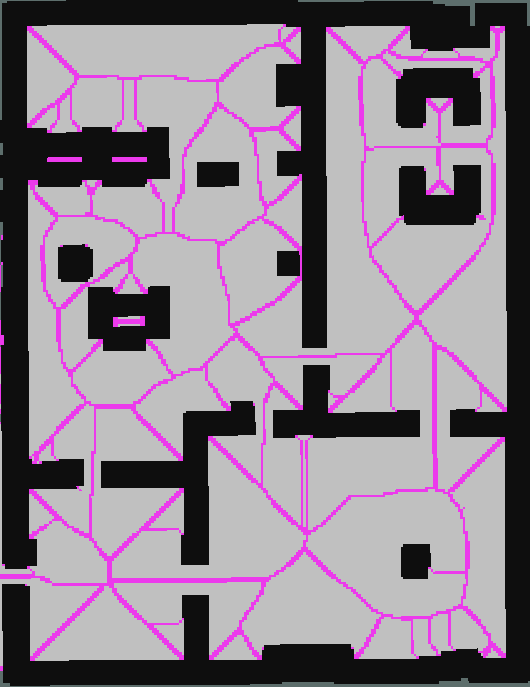
\includegraphics[width=\textwidth]{Figures/MotionPlanning/GVDFromGrid.png}
    \end{column}
  \end{columns}
\end{frame}

\section{Planeación de rutas}
\begin{frame}\frametitle{Planeación de rutas}
  La planeación de rutas consiste en encontrar una secuencia de configuraciones $q\in Q_{free}$ que permitan al robot moverse desde una configuración inicial $q_{start}$ hasta una configuración final $q_{goal}$.
  \begin{itemize}
  \item Una \textbf{ruta} es solo la secuencia de configuraciones para llegar a la meta.
  \item Cuando la secuencia de configuraciones se expresa en función del tiempo, entonces se tiene una \textbf{trayectoria}. 
  \end{itemize}
  En este curso solo vamos a hacer planeación de rutas, no de trayectorias (para navegación).\\
  Existen varios métodos para planear rutas. La mayoría de ellos se pueden agrupar en:
  \begin{itemize}
  \item Métodos basados en muestreo
  \item Métodos basados en grafos
  \end{itemize}
\end{frame}

\begin{frame}\frametitle{Métodos basados muestreo}
  Como su nombre lo indica, consisten en tomar muestras aleatorias del espacio libre. Si es posible llegar en línea recta de la configuración actual al punto muestrado, entonces se agrega a la ruta.
  Ejemplos:
  \begin{itemize}
  \item RRT (Rapidly-exploring Random Trees)
  \item RRT-Bidireccional
  \item RRT-Extendido
  \end{itemize}
\end{frame}

\begin{frame}\frametitle{\textit{Rapidly-exploring Random Trees}}
  Consiste en construir un árbol a partir de muestras aleatorias del espacio libre. Los pasos generales se pueden resumir en:
  \begin{columns}
    \begin{column}{0.55\textwidth}
      \begin{enumerate}
      \item Construir un árbol $T$ con nodo raíz en el punto inicial
      \item Elegir una posición aleatoria $p=(x,y)$ dentro del espacio libre
      \item Encontrar el nodo $n$, del árbol $T$, más cercano al punto $p$
      \item Si la distancia $d(n, p) > \epsilon$, cambiar $p$ por un punto en la misma dirección $\overrightarrow{np}$ pero a una distancia $\epsilon$
      \item Si no hay colisión entre $n$ y $p$, agregar a $p$ como nodo hijo de $n$
      \item Si no hay colisión entre $p$ y el punto meta $p_g$, agregar $p_g$ como nodo hijo de $p$, terminar la exploración y anunciar éxito
      \item Repertir desde el punto 2 un máximo de $N$ veces.
      \end{enumerate}
    \end{column}
    \begin{column}{0.45\textwidth}
      \begin{figure}
        \centering
        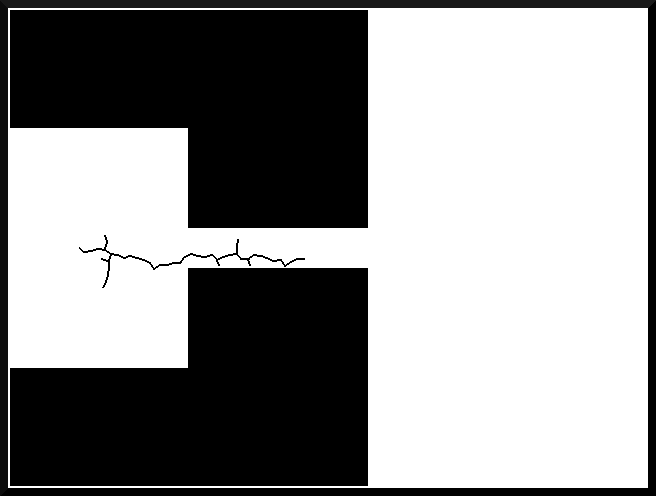
\includegraphics[width=0.45\textwidth]{Figures/MotionPlanning/RRTO010.png}
        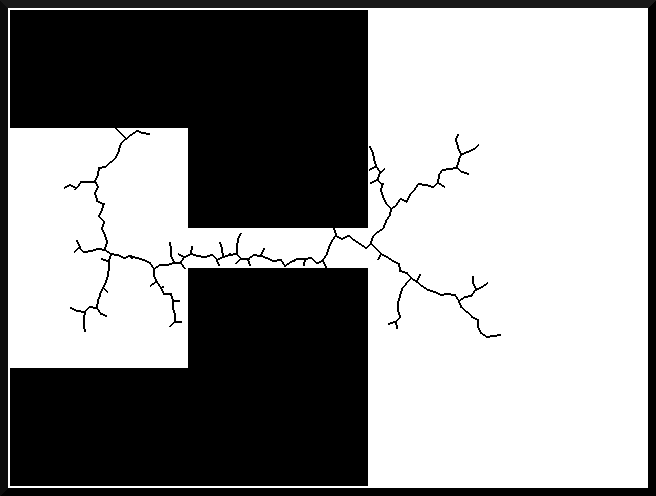
\includegraphics[width=0.45\textwidth]{Figures/MotionPlanning/RRTO0100.png}
        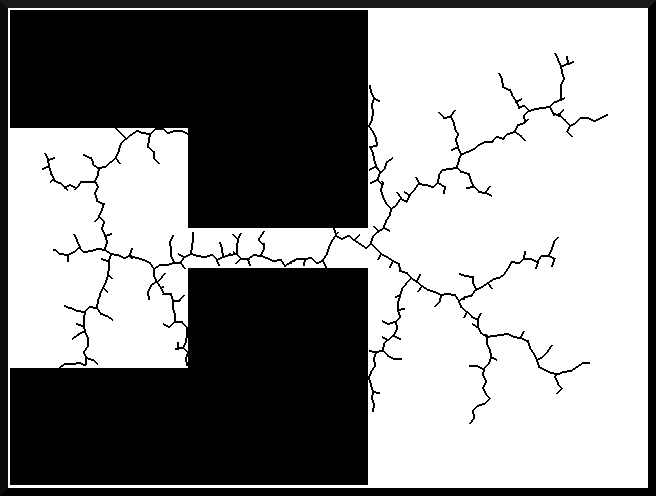
\includegraphics[width=0.45\textwidth]{Figures/MotionPlanning/RRTO0300.png}
      \end{figure}
    \end{column}
  \end{columns}
\end{frame}

\begin{frame}\frametitle{Métodos basados en grafos}
  Estos métodos consideran el ambiente como un grafo. En el caso de celdas de ocupación, cada celda libre es un nodo que está conectado con las celdas vecinas que también estén libres. Los pasos generales de este tipo de algorimos se pueden resumir en:
  \[\]
  \begin{algorithm}[H]
    \footnotesize
    \DontPrintSemicolon
    \KwData {Mapa $M$ de celdas de ocupación, configuración inicial $q_{start}$, configuración meta $q_{goal}$}
    \KwResult{Ruta $P=[q_{start},q_1, q_2, \dots , q_{goal}]$}
    Obtener los nodos $n_s$ y $n_g$ correspondientes a $q_{start}$ y $q_{goal}$\;
    Lista abierta $OL = \emptyset$ y lista cerrada $CL = \emptyset$\;
    Agregar $n_s$ a $OL$\;
    Nodo actual $n_c = n_s$\;
    \While{$OL\neq \emptyset$ y $n_c\neq n_g$}
    {
      Seleccionar $n_c$ de $OL$ \textbf{bajo algún criterio}\;
      Agregar $n_c$ a $CL$\;
      Expandir $n_c$\;
      Agregar a $OL$ los vecinos de $n_c$ que no estén ya en $OL$ ni en $CL$\;
    }
    \If{$n_c\neq n_g$}{Anunciar Falla}
    Obtener la configuración $q_i$ para cada nodo $n_i$ de la ruta\;
  \end{algorithm}
\end{frame}

\begin{frame}\frametitle{Métodos basados en grafos}
  El criterio para seleccionar el siguiente nodo a expandir $n_c$ de la lista abierta, determina el tipo de algoritmo:
  \begin{itemize}
  \item Criterio FIFO: Búsqueda a lo ancho BFS (la lista abierta es una cola)
  \item Criterio LIFO:  Búsqueda en profundidad DFS (la lista abierta es una pila)
  \item Menor valor $g$: Dijkstra (la lista abierta es una cola con prioridad)
  \item Menor valor $f$: A* (la lista abierta es una cola con prioridad)
  \end{itemize}
  Si el costo $g$ para ir de una celda a otra es siempre 1, entonces Dijkstra es equivalente a BFS. \\
  A* y Dijkstra siempre calculan la misma ruta (óptima) pero A* lo hace más rápido. 
\end{frame}

\begin{frame}\frametitle{Mapas de costo}
  \begin{itemize}
  \item Los métodos como Dijkstra y A* minimizan una función de costo. Esta función podría ser distancia, tiempo de recorrido, número de giros, energía gastada, entre otras.
  \item En este curso se empleará como costo una combinación de distancia recorrida más peligro de colisión (cercanía a los obstáculos).
  \item De este modo, las rutas serán un equilibrio entre rutas cortas y rutas seguras.
  \item Ejemplo: la ruta azul es más larga pero más segura. 
  \end{itemize}
  \begin{figure}
    \centering
    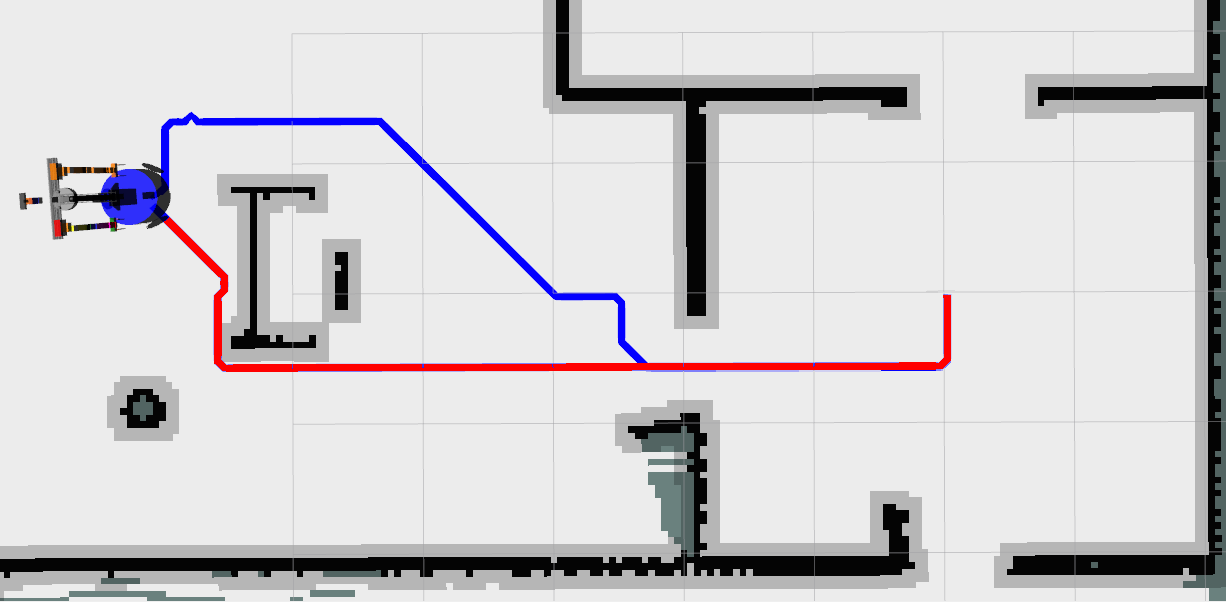
\includegraphics[width=0.5\textwidth]{Figures/MotionPlanning/AStarComparison.png}
  \end{figure}
\end{frame}

\begin{frame}\frametitle{Mapas de costo}
  \begin{itemize}
  \item Se utilizará como costo una función de \textit{cercanía}.
  \item Se calcula de forma similar al algoritmo Brushfire, pero la función decrece conforme nos alejamos de los objetos. 
  \end{itemize}
  \begin{columns}
    \begin{column}{0.6\textwidth}
      \begin{algorithm}[H]
        \footnotesize
        \DontPrintSemicolon
        \KwData {\;
          Mapa $M$ de celdas de ocupación\;
          Radio de costo $r_c$
        }
        \KwResult{Mapa de costo $M_c$}
        \;
        $M_c = $ Copia de $M$\;
        \ForEach{$i\in [0,\dots,rows)$}
        {
          \ForEach{$j\in [0,\dots,cols)$}
          {
            //Si está ocupada, calcular el costo de $r_c$ celdas alrededor.\;
            \If{$M[i,j] == 100$ }
            {
              \ForEach{$k_1\in [-r_c,\dots,r_c]$}
              {
                \ForEach{$k_2\in [-r_c,\dots,r_c]$}
                {
                  $C = r_c - max(|k1|,|k2|) + 1$\;
                  $M_c[i+k1,j+k2] = max(C, M_c[i+k1,j+k2]$\;
                }
              }
            }    
          }
        }
        \caption{Mapa de costo}
      \end{algorithm}
    \end{column}
    \begin{column}{0.4\textwidth}
      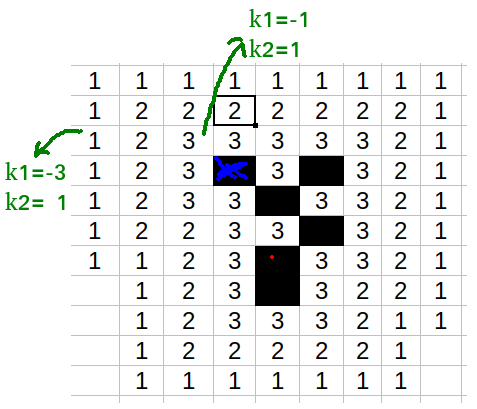
\includegraphics[width=0.95\textwidth]{Figures/MotionPlanning/CostMap.png}
    \end{column}
  \end{columns}
\end{frame}

\begin{frame}\frametitle{El algoritmo A*}
  \begin{itemize}
  \item Es un algoritmo completo, es decir, si la ruta existe, seguro la encontrará, y si no existe, lo indicará en tiempo finito.
  \item Al igual que Dijkstra, A* encuentra una ruta que minimiza una función de costo, es decir, es un algoritmo óptimo.
  \item Es un algoritmo del tipo de búsqueda informada, es decir, utiliza información sobre el estimado del costo restante para llegar a la meta para priorizar la expansión de ciertos nodos. 
  \item El nodo a expandir se selecciona de acuerdo con la función:
    \[f(n) = g(n) + h(n)\]
    donde
    \begin{itemize}
    \item $g(n)$ es el costo acumulado del nodo $n$
    \item $h(n)$ es una función heurística que \textbf{subestima} el costo de llegar del nodo $n$ al nodo meta $n_g$. 
    \end{itemize}
  \item Se tienen los siguientes conjuntos importantes:
    \begin{itemize}
    \item Lista abierta: conjunto de todos los nodos en la frontera (visitados pero no conocidos). Es una cola con prioridad donde los elementos son los nodos y la prioridad es el valor $f(n)$.
    \item Lista cerrada: conjunto de nodos para los cuales se ha calculado una ruta óptima. 
    \end{itemize}
    \item A cada nodo se asocia un valor $g(n)$, un valor $f(n)$ y un nodo padre $p(n)$. 
  \end{itemize}
\end{frame}

\begin{frame}\frametitle{El algoritmo A*}
    \begin{algorithm}[H]
    \footnotesize
    \DontPrintSemicolon
    \KwData {Mapa $M$, nodo inicial $n_s$ con configuración $q_{s}$, nodo meta $n_g$ con configuración $q_{g}$}
    \KwResult{Ruta óptima $P=[q_{s},q_1, q_2, \dots , q_{g}]$}
    Lista abierta $OL = \emptyset$ y lista cerrada $CL = \emptyset$\;
    Fijar $f(n_{s}) = 0$, $g(n_{s}) = 0$ y $prev(n_{s}) = NULL$\;
    Agregar $n_s$ a $OL$ y fijar nodo actual $n_c = n_s$\;
    \While{$OL\neq \emptyset$ y $n_c\neq n_g$}
    {
      Remover de $OL$ el nodo $n_c$ con el menor valor $f$ y agregar $n_c$ a $CL$\;
      \ForAll{$n$ vecino de $n_c$}
      {
        $g = g(n_c) + costo(n_c, n)$\;
        \If{$g < g(n)$}
        {
          $g(n) = g$\;
          $f(n) = h(n) + g(n)$\;
          $prev(n) = n_c$\;
        }
      }
      Agregar a $OL$ los vecinos de $n_c$ que no estén ya en $OL$ ni en $CL$\;
    }
    \If{$n_c\neq n_g$}{Anunciar Falla}
    \While{$n_c \neq NULL$}
    {
      Insertar al inicio de la ruta $P$ la configuración correspondiente al nodo $n_c$\;
      $n_c = prev(n_c)$
    }
    Devolver ruta óptima $P$
  \end{algorithm}
\end{frame}

\begin{frame}\frametitle{El algoritmo A*}
  \begin{itemize}
  \item La función de costo será el número de celdas más el mapa de costo obtenido anteriormente.
  \item Puesto que el mapa está compuesto por celdas de ocupación, los nodos vecinos se pueden obtener usando conectividad 4 o conectividad 8.
  \item Si se utiliza conectividad 4, la distancia de Manhattan es una buena heurística.
  \item Si se utiliza conectividad 8, se debe usar la distancia Euclideana.
  \item La lista abierta se puede implementar con una \textit{Heap}, de este modo, la inserción de los nodos $n$ se puede hacer en tiempo logarítmico y la selección del nodo con menor $f$ se hace en tiempo constante.
  \end{itemize}
\end{frame}

\section{Seguimiento de rutas}
\begin{frame}\frametitle{Seguimiento de rutas}
  Hasta el momento ya se tiene una representación del ambiente y una forma de planear rutas. Ahora falta diseñar las leyes de control que hagan que el robot se mueva por la ruta calculada. Este control se hará bajo los siguientes supuestos:
  \begin{itemize}
  \item Se conoce la posición del robot (más adelante se abodará el problema de la localización)
  \item El modelo cinemático es suficiente para modelar el movimiento del robot 
  \item Las dinámicas no modeladas (parte eléctrica y mecánica de los motores) son lo suficientemente rápidas para poder despreciarse
  \end{itemize}
\end{frame}

\begin{frame}\frametitle{Base diferencial}
  \begin{itemize}
  \item Es la configuración más sencilla debido a la simplicidad del hardware requerido
  \item Aunque implica restricciones no holonómicas, es suficiente para la mayoría de los movimientos requeridos. Además, suponer este tipo de base es algo útil debido a una razón sencilla: los sensores suelen estar al frente del robot. 
  \item Se diseñarán leyes de control suponiendo esta configuración.
  \end{itemize}
  \begin{columns}
    \begin{column}{0.4\textwidth}
      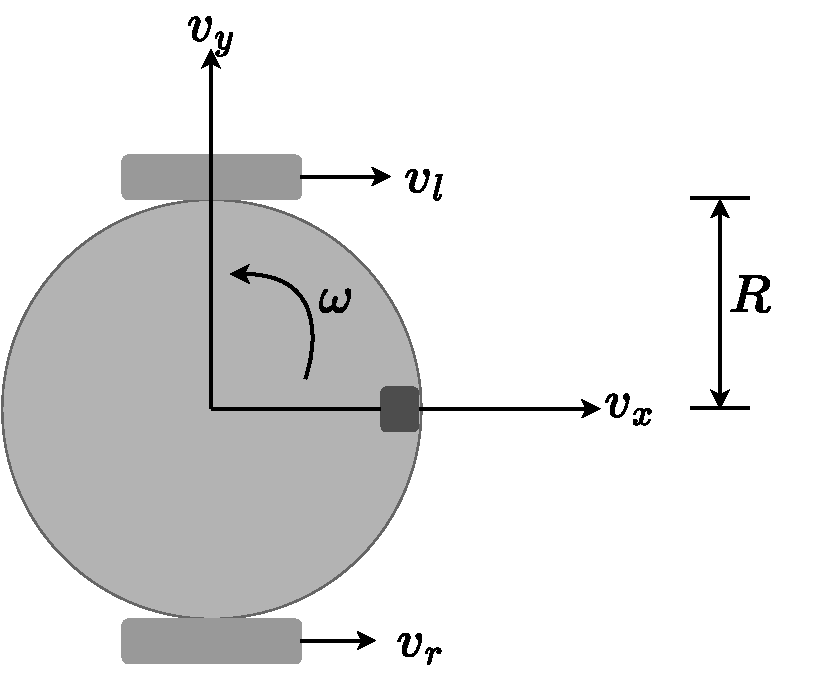
\includegraphics[width=\textwidth]{Figures/MotionPlanning/DifferentialBase.pdf}
    \end{column}
    \begin{column}{0.6\textwidth}
      \begin{eqnarray*}
        v_l &=& v_x - R\omega\\
        v_r &=& v_x + R\omega
      \end{eqnarray*}
    \end{column}
  \end{columns}
\end{frame}

\begin{frame}\frametitle{Position control}
  \begin{columns}
    \begin{column}{0.5\textwidth}
      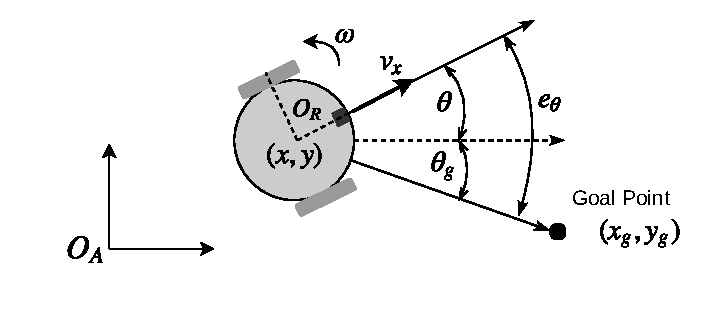
\includegraphics[width=0.95\textwidth]{Figures/MotionPlanning/GoalPose.pdf}
    \end{column}
    \begin{column}{0.5\textwidth}
      Considere una base diferencial y el punto meta $(x_g, y_g)$, las siguientes leyes de control permiten al robot alcanzar dicho punto meta:
      \begin{eqnarray*}
        v_x    &=& v_{max}e^{-\frac{e_{\theta}^{2}}{\alpha}}\label{eq:Control11}\\
        \omega &=& \omega_{max}\left(\frac{2}{1+e^{-\frac{e_{\theta}}{\beta}}}-1\right)\label{eq:Control12}
      \end{eqnarray*}
    \end{column}
  \end{columns}
  con
  \[e_{\theta} = \atantwo\left(y_g - y, x_g - x\right) - \theta\]
  El error de ángulo $e_\theta$ debe estar siempre en $(-\pi, \pi]$. If the resulting value is out this interval, angle can be wraped with:
  \[e_\theta \leftarrow \left(e_\theta + \pi\right)\% (2\pi) - \pi\]
  where \% denotes the module operator. 
\end{frame}

\begin{frame}\frametitle{Position control}
  \begin{itemize}
  \item $v_{max}$ and $\omega_{max}$ are the maximum linear and angular speed and depend on the physical capabilities of the mobile base.
  \item $\alpha$ and $\beta$ determine how fast linear and angular speed change when angle error changes.
  \item In general, small values of $\alpha$ and $\beta$ make the robot to follow the path more accurately but too small values can cause chattering.
    \item Big values of  $\alpha$ and $\beta$ produce a smoother movement but can result in very extense curves. 
  \end{itemize}
  \begin{figure}
    \centering
    \includegraphics[width=0.45\textwidth]{Figures/MotionPlanning/LinearSpeed.eps}
    \includegraphics[width=0.45\textwidth]{Figures/MotionPlanning/AngularSpeed.eps}
  \end{figure}
\end{frame}


\begin{frame}\frametitle{Speed profile}
  \begin{columns}
    \begin{column}{0.43\textwidth}
      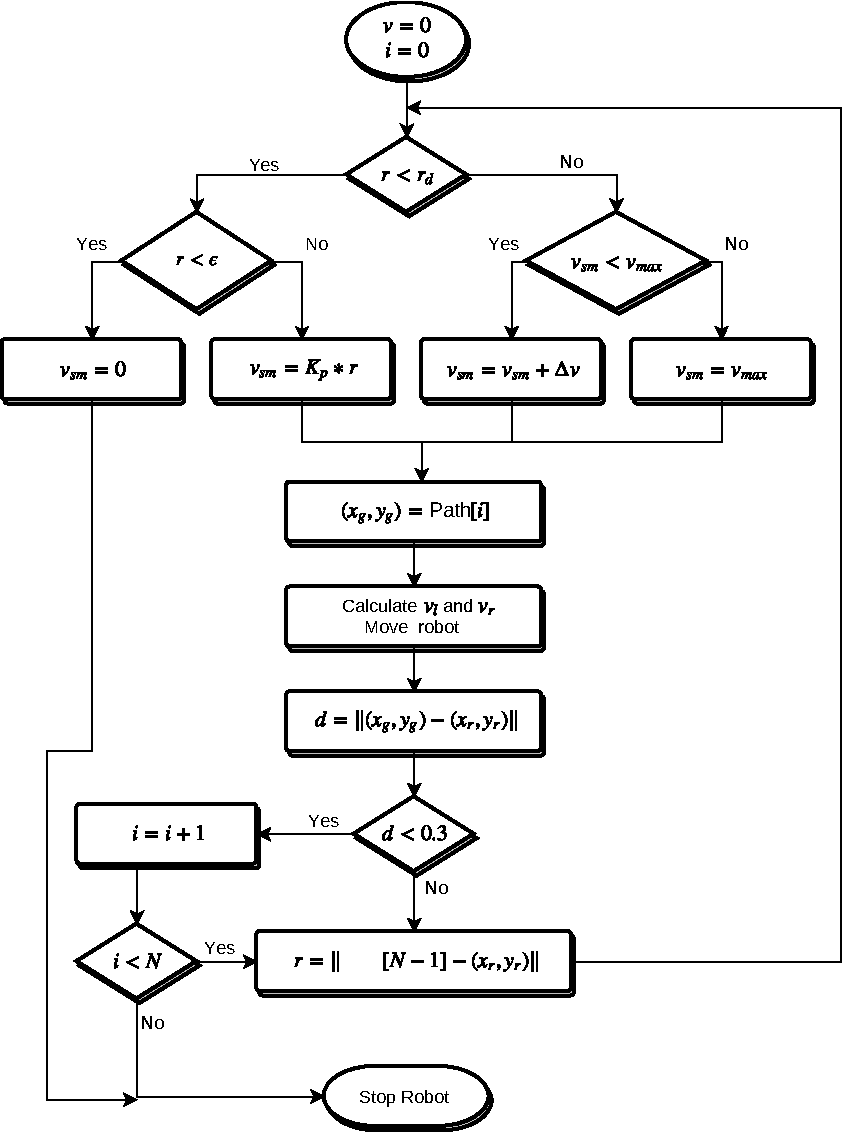
\includegraphics[width=\textwidth]{Figures/MotionPlanning/AFSM.pdf}
    \end{column}
    \begin{column}{0.5\textwidth}
      Consider a finite state machine to calculate $v_{max}$. Let $v_{sm}$ be the new max linear speed, such that, now the control law is given by:
      \begin{eqnarray*}
        v      &=& v_{sm}e^{-\frac{e_{\theta}^{2}}{\alpha}}\label{eq:NewControl1}\\
        \omega &=& \omega_{max}\left(\frac{2}{1+e^{-\frac{e_{\theta}}{\beta}}}-1\right)\label{eq:NewControl2}
      \end{eqnarray*}
      with
      \begin{itemize}
      \item $r$: Distance to global goal
      \item $\epsilon$: Tolerance to consider the robot has reached the global goal
      \item $r_d$: Distance to global goal to start decceleration
      \item $\Delta v$: Desired acceleration
      \end{itemize}
    \end{column}
  \end{columns}
\end{frame}

\begin{frame}\frametitle{Speed profile}
  The figure show an example of the planned path and the linear speeds generated using only the control laws and using the finite state machine to generate a profile speed. 
  \begin{figure}
    \centering
    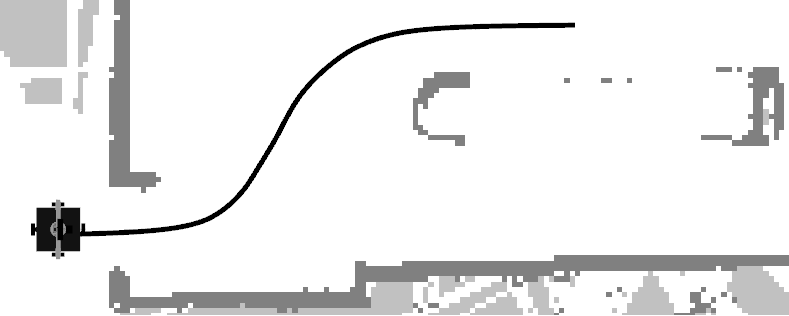
\includegraphics[width=0.45\textwidth]{Figures/MotionPlanning/SpeedProfilePath.png}
  \end{figure}
  \begin{figure}
    \centering
    \includegraphics[width=0.45\textwidth]{Figures/MotionPlanning/SpeedWithoutProfile.eps}
    \includegraphics[width=0.45\textwidth]{Figures/MotionPlanning/SpeedWithProfile.eps}
  \end{figure}
\end{frame}

\section{Path smoothing}
\begin{frame}\frametitle{Path smoothing}
  \begin{itemize}
  \item Since planned paths come from occupancy grids, they all have corners.
  \item Such corners can cause big changes in control laws and can lead to actuator damage.
  \item Green path in the figure shows a path planned with A *, nevertheless, it is preferable a path like the blue one.
  \end{itemize}
  \begin{figure}
    \centering
    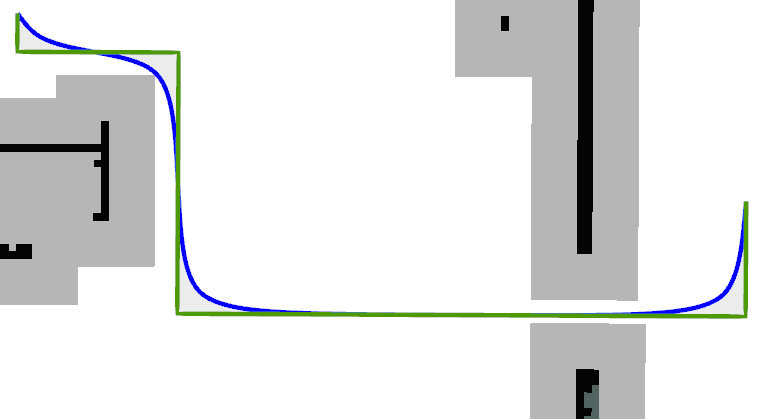
\includegraphics[height=0.45\textheight]{Figures/MotionPlanning/PathSmoothingExample.png}
  \end{figure}
  We will use an optimazion approach to smooth the A* path.
\end{frame}

\begin{frame}\frametitle{Smoothing by gradient descend}
  We propose to design a cost function such that minimizing such function will result in a smooth path. Black points represent the A* path with points $Q=\{q_0, q_1, \dots, q_n\}$ and blue points represent a smooth path with points $P=\{p_0, p_1,\dots, p_n\}$.
  \begin{columns}
    \begin{column}{0.5\textwidth}
      \begin{figure}
        \centering
        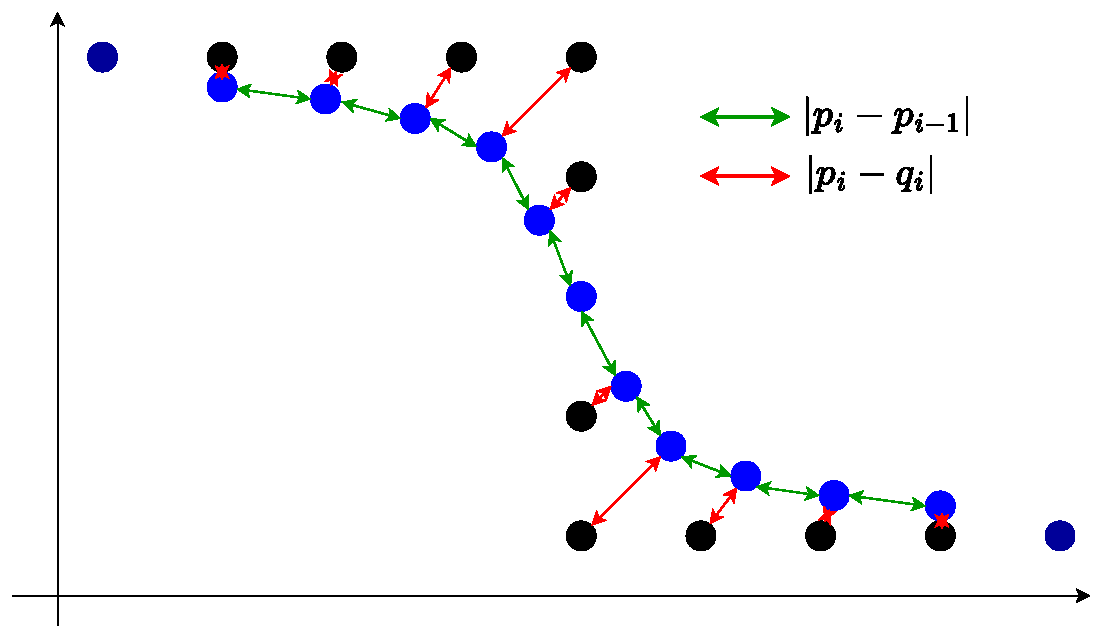
\includegraphics[width=\textwidth]{Figures/MotionPlanning/PathSmoothing.pdf}
      \end{figure}
    \end{column}
    \begin{column}{0.5\textwidth}
      Consider the cost function
      \[J = \alpha\frac{1}{2}\sum_{i=1}^{n-1}\left(p_i - p_{i-1}\right)^2 + \beta\frac{1}{2}\sum_{i=1}^{n-1}(p_i - q_i)^2\]
      \begin{itemize}
      \item $J$ is the sum of distances between a point in the smooth path and its corresponding point in the original path, plus the distances between consecutive point in the smooth path. 
      \item If the path is too smooth,$J$ will increase
      \item If the path is too similar to the original one, $J$ will also increase
      \item A path that minimizes $J$ will be both smooth and similar to the original one. 
      \end{itemize}
    \end{column}
  \end{columns}
\end{frame}

\begin{frame}\frametitle{Path smoothin by gradient descend}
  The minimum of function $J$ can be found by the gradient descend algorithm:
  \begin{algorithm}[H]
    \footnotesize
  \DontPrintSemicolon
  \KwData {Cost function $J(p):\mathbb{R}^n\rightarrow \mathbb{R}$ whose minimum is required}
  \KwResult{Vector $p$ that minimizes $J$}
  $p\leftarrow p_{init}$ //Set an initial guess\;
  \While{$|\nabla J(p)| > tol$}
  {
    $p \leftarrow p - \epsilon \nabla J (p)$ //$p$ is modified a little bit in the opposite direction to gradient.\;
  }
  Return  $p$
  \caption{Gradien descend}
\end{algorithm}
\[\]
Gradient descend finds the local minimum nearest to initial guess $p_0$, nevertheless, since cost function $J$ is quadratic, it has only a global minimum. Gradient of cost function $J$ is calculated as:
  \[\underbrace{\left[\frac{}{}\alpha(p_0 - p_1)+\beta(p_0 - q_0)\right. }_{\dfrac{\partial J}{\partial p_0}}
,\dots ,
\underbrace{\frac{}{}\alpha(2p_i - p_{i-1} - p_{i+1})+\beta(p_i - q_i)}_{\dfrac{\partial J}{\partial p_i}}
,\dots ,
\underbrace{\left.\alpha(p_{n-1} - p_{n-2})+\beta(p_{n-1}-q_{n-1})\frac{}{}\right]}_{\dfrac{\partial J}{\partial p_{n-1}}}
\]
\end{frame}

\begin{frame}\frametitle{Path smoothing by gradient descend}
  To keep start and goal points in the same value, first and las components of $\nabla J$ will be set to zero. The gradient descend algorithm can be summarized as follows:
  \[\]
\begin{algorithm}[H]
\DontPrintSemicolon
  \DontPrintSemicolon
  \KwData{Original A* path with points $Q = \{q_0\dots q_i \dots q_{n-1}\}$, parameters $\alpha$ and $\beta$, constant rate $\epsilon$ and tolerance $tol$\;}
  \KwResult{Smooth path with points $P = \{p_0\dots p_i \dots p_{n-1}\}$\;}
  $P \leftarrow Q$\;
  $\nabla J_0 \leftarrow 0$\;
  $\nabla J_{n-1} \leftarrow 0$\;   
  \While{ $\Vert\nabla J(p_i)\Vert > tol \wedge$ steps < max\_steps}
  {
    \ForEach{$i \in [1,n-1)$}
    {
      $\nabla J_i \leftarrow \alpha (2p_i - p_{i-1} - p_{i+1}) + \beta (p_i - q_i)$\;
    }
    $P \leftarrow P - \epsilon \nabla J$\;
    $steps \leftarrow steps + 1$
  }
  Return $P$
  \caption{Path smoothing with gradient descend}
\end{algorithm}
\end{frame}

\section{Obstacle avoidance}
\begin{frame}\frametitle{Artificial potential fields}
  The idea of this technique is to design a function $U(q):\mathbb{R}^n\rightarrow \mathbb{R}$ such that it represents potential energy.
  \begin{itemize}
  \item Gradient $\nabla U(q) = \left[\frac{\partial U}{\partial q_1},\dots,\frac{\partial U}{\partial q_n}\right]$ is a force vector
  \item It should be designed with a global minimum in the goal point and local maxima in every obstacle.
  \item If robot moves always in the opposite direction of gradient $\nabla U$, it will reach to goal point while avoiding obstacles. 
  \item $U(q)$ can be designed in several ways:
    \begin{itemize}
    \item \textit{wavefront} algorithm, which requires a discretization of the space (requires a map), but it does not have the problem of local minima.
    \item Attractive and rejection fields, which require no previous map nor discretization, but can have local minima. 
    \end{itemize}
  \end{itemize}
\end{frame}

\begin{frame}\frametitle{Attractive and rejection fields}
  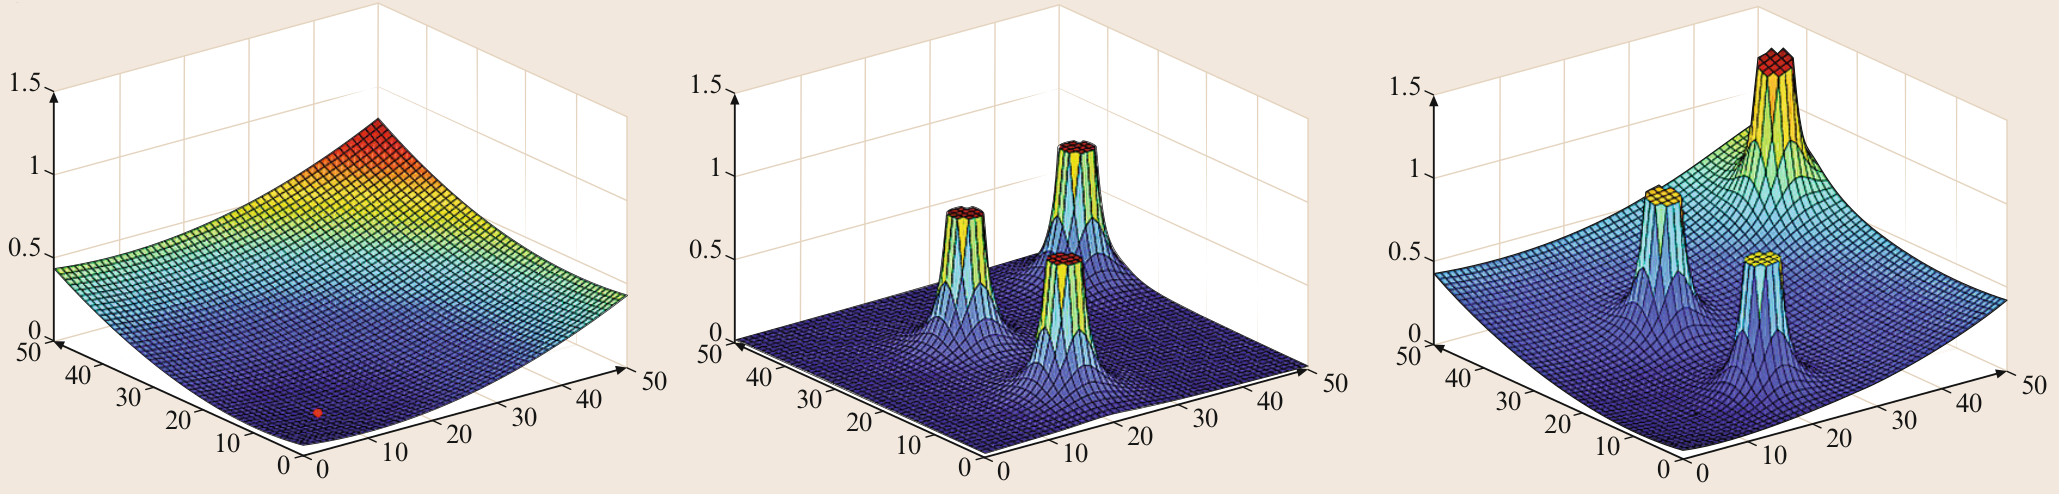
\includegraphics[width=\textwidth]{Figures/MotionPlanning/PotFieldsExample.png}
  \begin{itemize}
  \item \textbf{Rejection fields:} A function $U_{rej_i}(q)$ is designed for each obstacle with a local maximum at obstacle's position $q_{o_i}$. Gradient of this function should increase as we approach to obstacle and also, it should be small enough (or zero) when robot is far enough.
  \item \textbf{Attractive field:} A function $U_{att}(q)$ with a local minimum at goal point $q_g$.
  \item Total potential function  $U(q)$ is calculate as:
    \[ U(q) = U_{att}(q) + \frac{1}{N}\sum_{i=1}^N U_{rej_i}(q)\]
  \end{itemize}
\end{frame}

\begin{frame}\frametitle{Attrative and rejection forces}
  Since gradient is a linear operator, we can design directly the attractive $F_{att}(q) = \nabla U_{att}(q)$ and rejection $F_{rej_i}(q) = \nabla U_{rej_i}(q)$ forces, such that the total force will be:
  \[ \nabla U(q) = F(q) = F_{att}(q) + \frac{1}{N}\sum_{i=1}^N F_{rej_i}(q)\]
  A proposal for this forces is:
  \begin{eqnarray*}
    \label{eq:attractive}
    F_{att} &=& \eta \dfrac{\left(q - q_g\right) }{\Vert q - q_g \Vert},\qquad \zeta > 0\label{eq:PotFieldsAttraction}\\
    F_{rej} &=& \begin{cases}
                  \zeta\left(\sqrt{\dfrac{1}{d} - \dfrac{1}{d_0}}\right)\dfrac{q_{o_i} - q}{d}
                  & \quad\textrm{si}\quad d < d_0\\
                  0 & \quad\textrm{en otro caso}
                \end{cases}
  \end{eqnarray*}
  where
  \begin{itemize}
  \item $q=(x,y)$ is the robot position
  \item $q_g=(x_g, y_g)$ is the goal point
  \item $q_{o_i} = (x_{o_i}, y_{o_i})$ is the position of $i$-th obstacle
  \item $d_0$ is a distance of influence. Obstacles farther than $d_0$ have no effect
  \item $\zeta$, $\eta$ and $d_0$ are tunning constants
  \end{itemize}
\end{frame}

\begin{frame}\frametitle{Obstacle avoidance by potential fields}
  \begin{itemize}
  \item Although previous equations assume that every obstacle's position $q_{o_i}$ is known, in fact, this position appears only in the difference $q_{o_i} - q$, i.e, it is required only the obstacle position w.r.t. robot.
  \item Potential fields are implemented using the lidar sensor, where each reading is considered as an obstacle. 
  \end{itemize}
  \begin{figure}
    \centering
    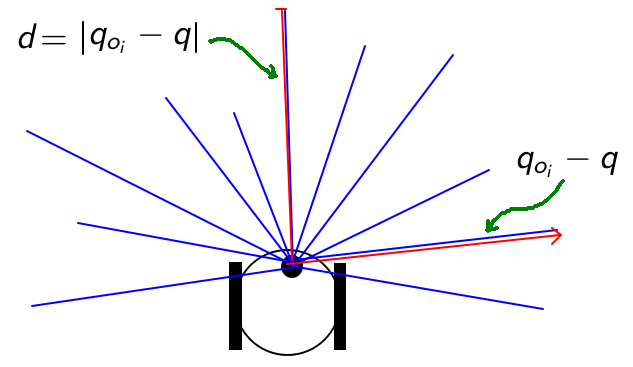
\includegraphics[width=0.4\textwidth]{Figures/MotionPlanning/PotFieldsLidar.png}
  \end{figure}
  Lidar readings are, in general, distance-angle pairs $(d_i,\theta_i)$, expressed w.r.t. robot, thus, if robot position $(x_r,y_r,\theta_r)$ is known, then each obstacle position can be calculated as:
  \begin{eqnarray*}
    x_{oi} &=& x_r + d_i\cos(\theta_i + \theta_r)\\
    y_{oi} &=& y_r + d_i\sin(\theta_i + \theta_r)\\
  \end{eqnarray*}
\end{frame}

\begin{frame}\frametitle{Obstacle avoidance by potential fields}
  Finally, in order to make the robot move towards goal point, we can use the gradient descend algorithm:
  \[\]
  \begin{algorithm}[H]
  \DontPrintSemicolon
  \KwData{Start position $q_s$, goal position $q_g$, obstacle positions $q_{oi}$ and tolerand $tol$}
  \KwResult{Sequence of points $\{q_0,q_1, q_2, \dots\}$ to reach the goal point and evade obstacles at the same time.}
  \;
$q \leftarrow q_s$\;
\While{$\Vert\nabla U(q)\Vert > tol$}
{
  $q \leftarrow q - \epsilon F(q)$\;
  $[v,\omega] \leftarrow $ control laws with $q$ as desired position\;
}
  \caption{Gradient descend to move the robot through a potential field}
  \label{alg:PotFields}
\end{algorithm}
\end{frame}

\begin{frame}\frametitle{Obstacle avoidance by potential fields}
  Figure shows an example of the movement achieved by potential fields:
  \begin{figure}
    \centering
    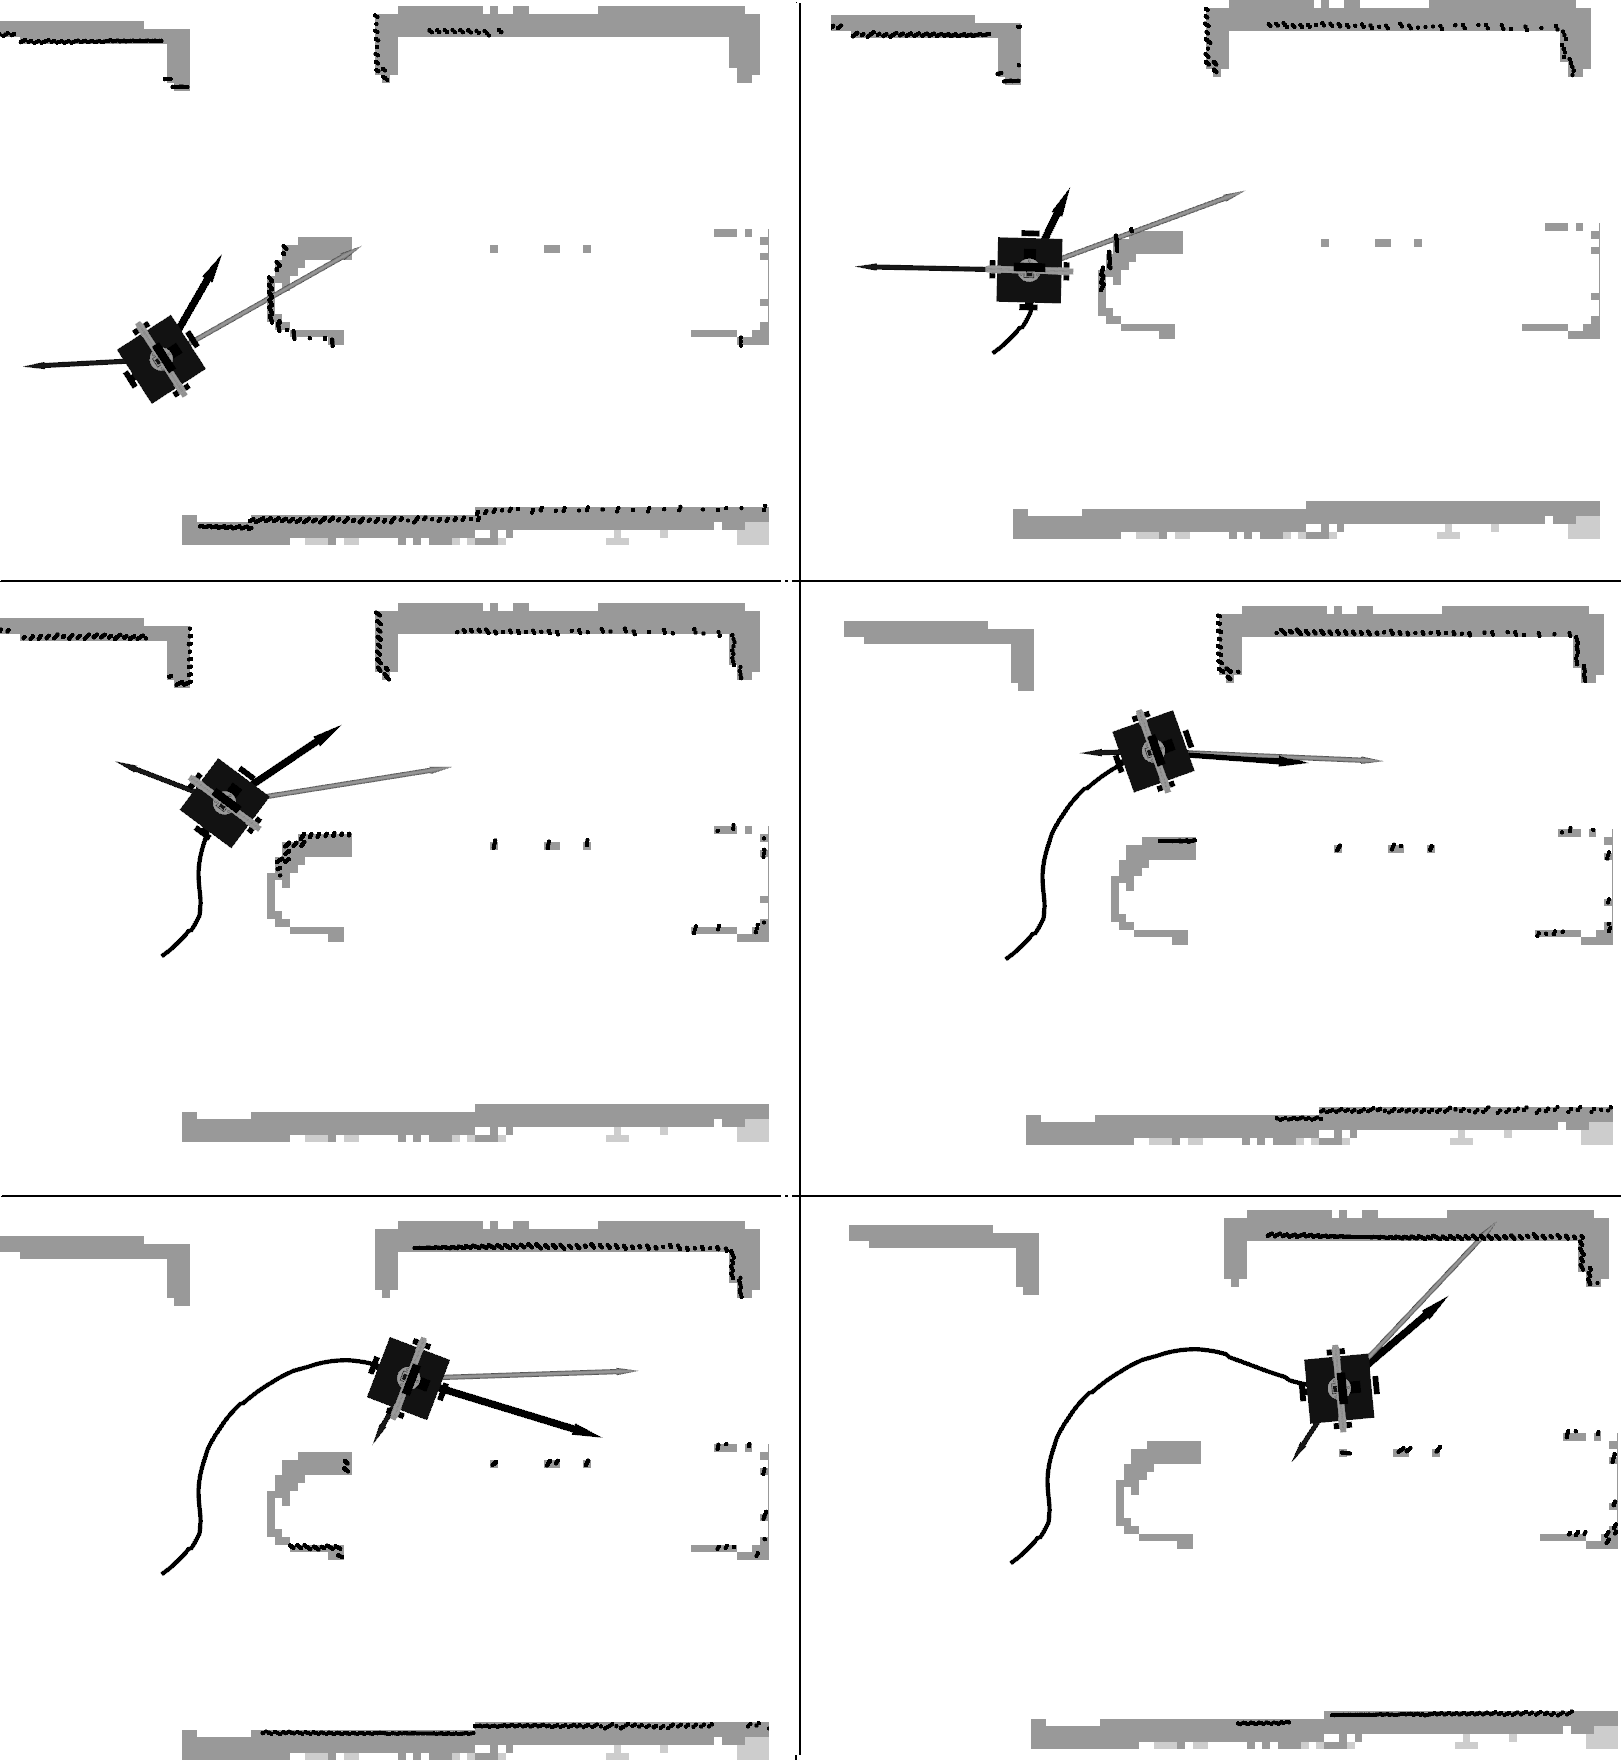
\includegraphics[height=0.85\textheight]{Figures/MotionPlanning/PotFieldsExecution.png}
  \end{figure}
\end{frame}

\begin{frame}\frametitle{Localization}
  The problem of localization consist on determine the robot configuration $q$ given a map and a set of sensor readings. uras de los sensores.
  \begin{itemize}
  \item Localization could be achieve by simply integrating robot speed commands, this method is known as odometry.
  \item If exact initial condition is known and the robot executes perfectly the movement commands, then odometry would be enough to localize the robot.
  \item This is of course not possible. There is uncertainty both in the robot movement and the initial condition, i.e., the robot looses information about its own position with every movement. 
  \end{itemize}
\end{frame}

\section{Localization}
\begin{frame}\frametitle{Localization}
  Methods can be classified in two types:
\[\]
  \begin{columns}
    \begin{column}{0.5\textwidth}
      \textbf{Local localization: }
      \begin{itemize}
      \item Requires an initial estimation \textit{close enough} to the real initial position, otherwise, localization does not converge.
      \item It is usually less expensive in term of computing cost.
      \item A common method is the Extended Kalman Filter
      \end{itemize}
    \end{column}
    \begin{column}{0.5\textwidth}
      \textbf{Global localization:}
      \begin{itemize}
      \item Initital guess can be any estimation
      \item It is usually very expensive in term of computing cost
      \item A common method is the particle filter
      \end{itemize}
      \[\]
      \[\]
    \end{column}
  \end{columns}
\end{frame}

\begin{frame}\frametitle{Particle filters}
  Localization by particle filters can be achieved with 5 general steps:
  \begin{enumerate}
  \item Generate a set of $N$ particles with random uniformly distributed $(x,y,\theta)$
  \item Move each particle a displacement  $(\Delta x, \Delta y, \Delta\theta)$ plus Gaussian noise
  \item Simulate lidar readings for each particle
  \item Compare each simulated reading with the real sensor reading. Similarities will represent a probability distribution.
  \item Resample $N$ particles, with replacement, using the previous probability distribution and add gaussian noise to each resampled particle. 
  \end{enumerate}
\end{frame}

\begin{frame}\frametitle{Particle Filters}
  \begin{figure}
    \centering
    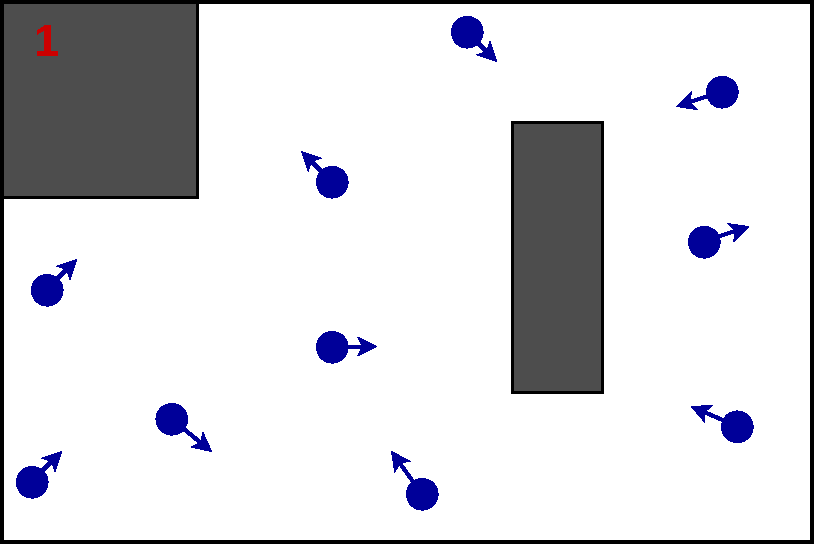
\includegraphics[width=0.30\textwidth]{Figures/MotionPlanning/ParticleFilter1.pdf}
    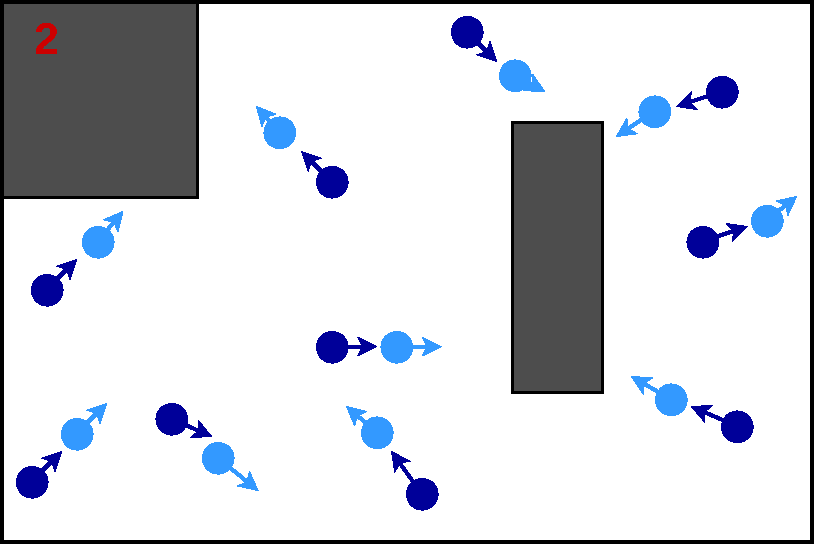
\includegraphics[width=0.30\textwidth]{Figures/MotionPlanning/ParticleFilter2.pdf}
    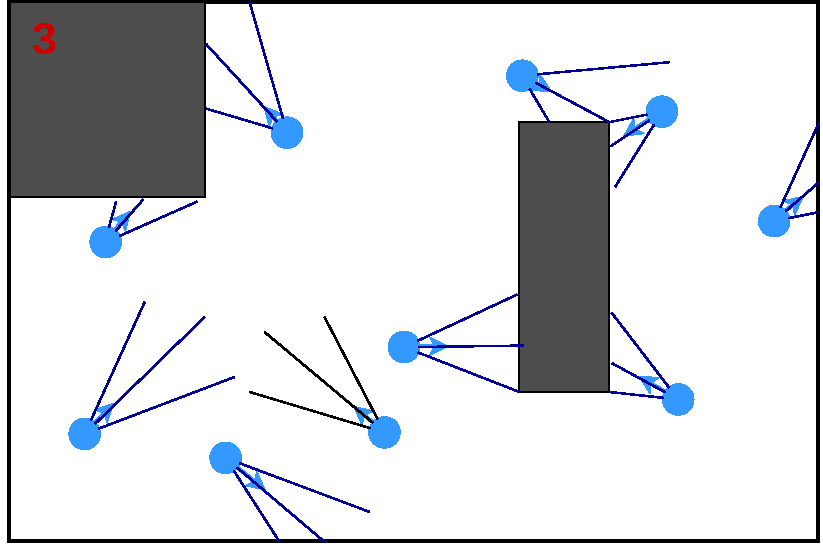
\includegraphics[width=0.30\textwidth]{Figures/MotionPlanning/ParticleFilter3.pdf}
    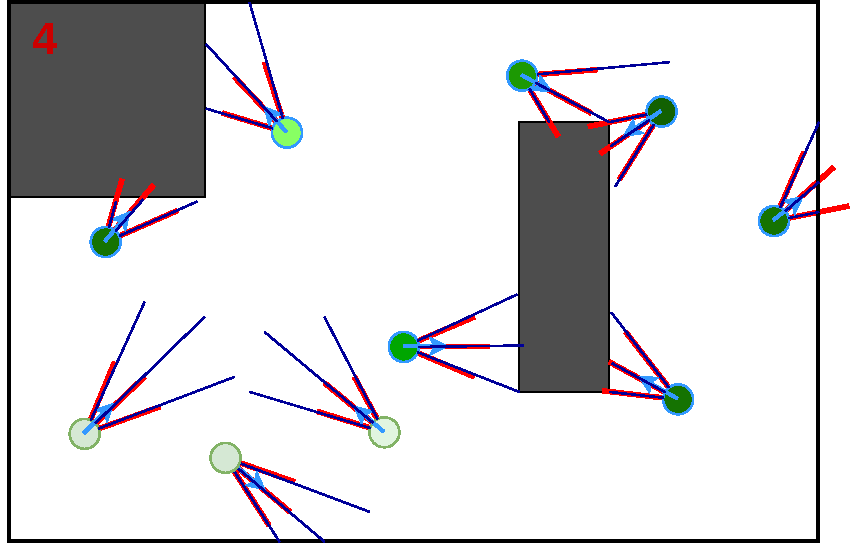
\includegraphics[width=0.31\textwidth]{Figures/MotionPlanning/ParticleFilter4.pdf}
    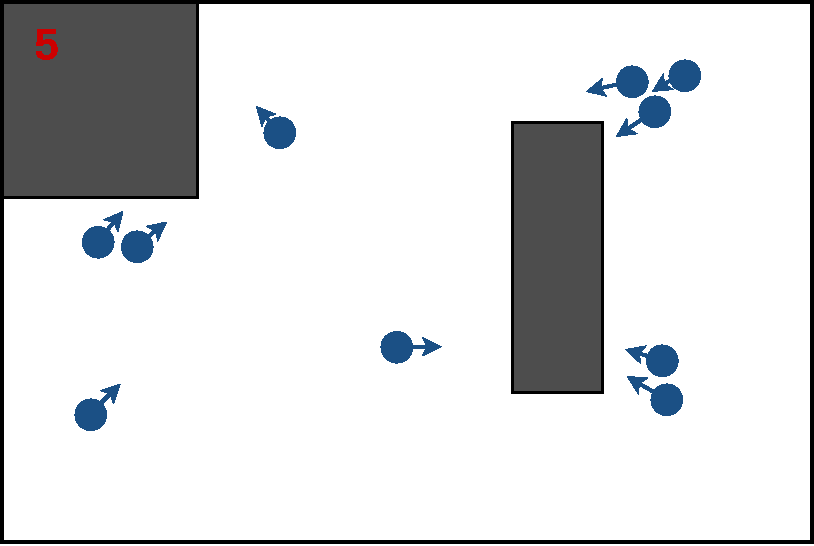
\includegraphics[width=0.30\textwidth]{Figures/MotionPlanning/ParticleFilter5.pdf}
  \end{figure}
\end{frame}
